% 第四章：面向硬件页表与位级并行的极坐标执行引擎（合并非对称投影/CJ-Gate/草图方差命题与系统算子实现）
\section{Hardware-Conscious Polar Execution Engine}
\label{sec:system}

\begin{figure*}[t]
  \centering
  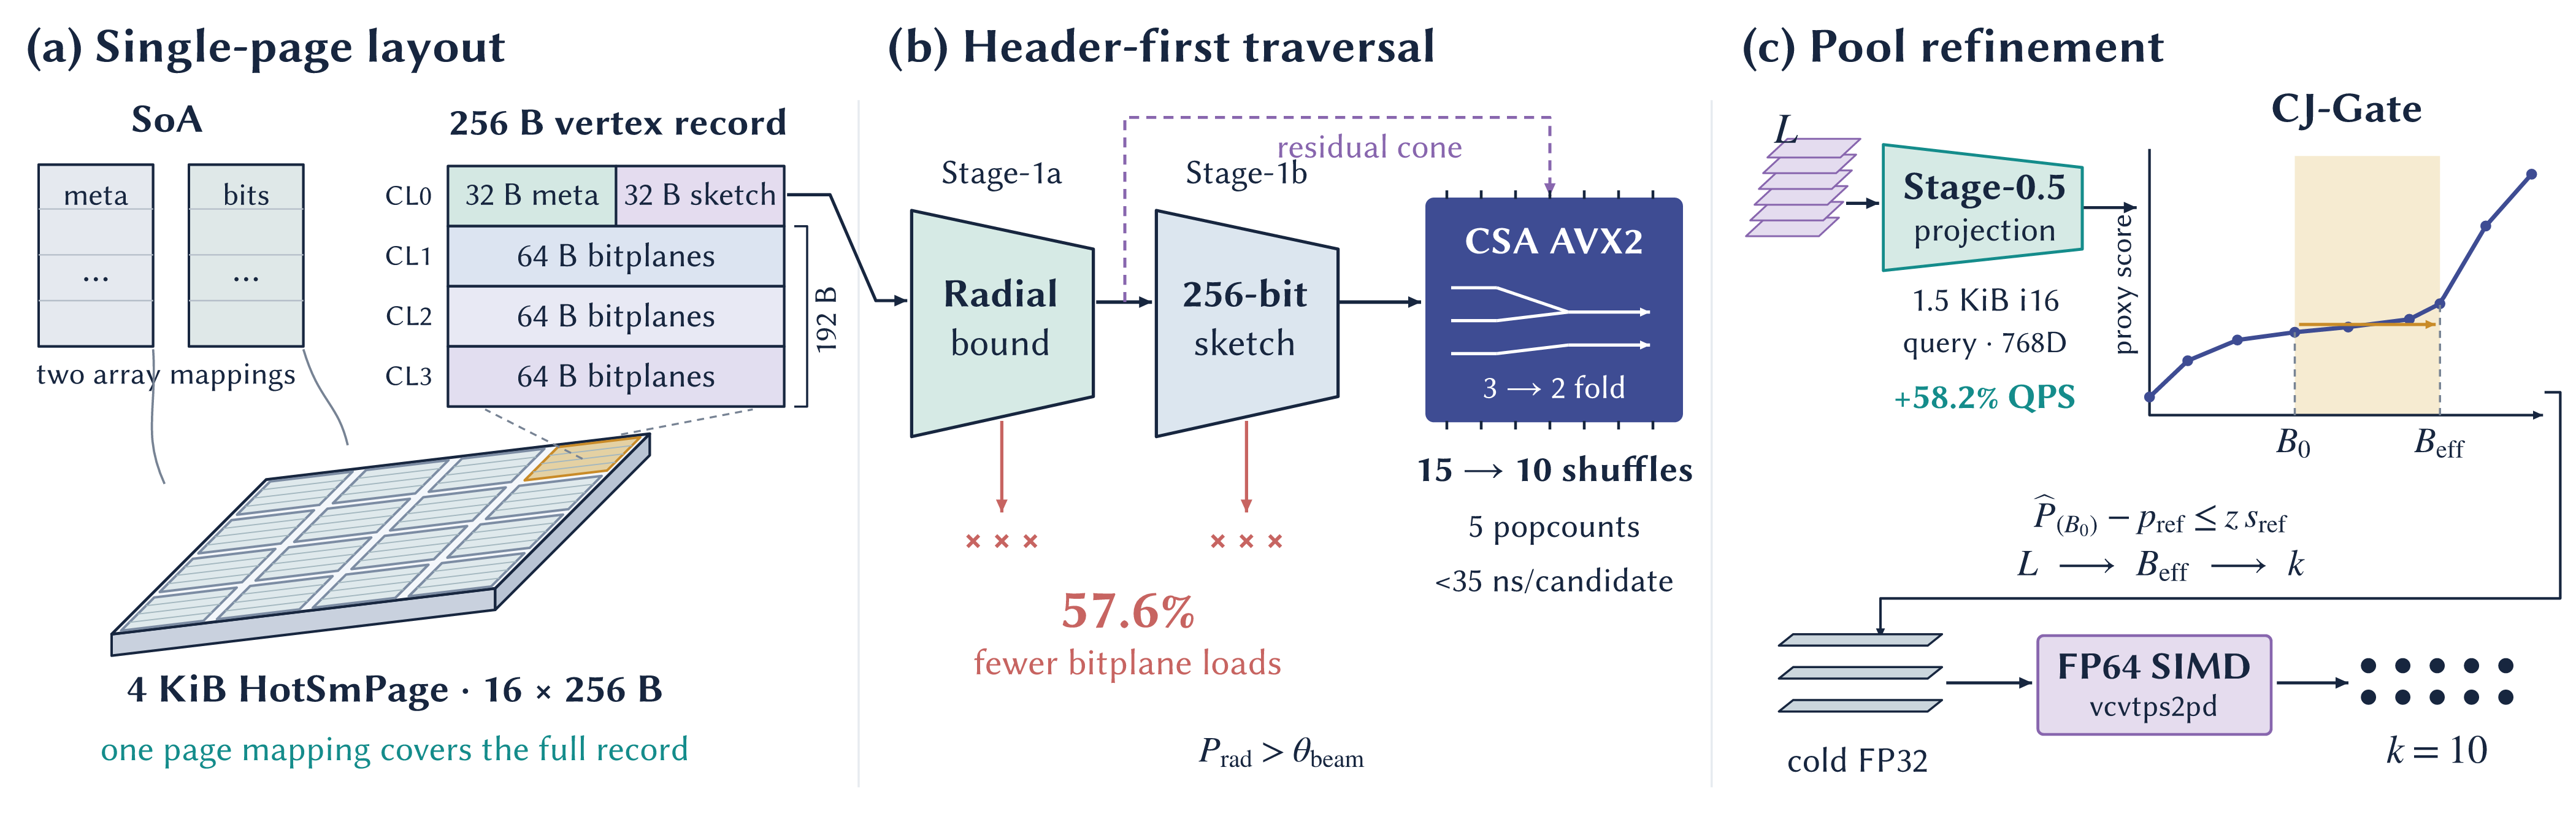
\includegraphics[width=\textwidth]{pelorus_execution.png}
  \caption{Header-first query execution at $D=768$. (a)~One $4$\,KiB page contains 16 records, each with a 64\,B header and 192\,B bitplanes. (b)~Radial and sketch gates precede full bitplane reads, with residual vertices bypassing the sketch gate. The skip rate and kernel annotations use the {Cohere-1M} measurements. (c)~Asymmetric projection precedes adaptive rerank admission and cold-vector FP64 evaluation. The score curve is schematic. \textsc{Stage-0.5} improves $99.5\%$-recall {Cohere} QPS by $58.2\%$ in the controlled ablation. The measured $+63.7\%$ ({Cohere}, $99.5\%$ recall) and $+76.5\%$ ({MERU}, $99\%$ recall) gains combine \textsc{CJ-Gate} with stabilized sketching.}
  \label{fig:execution_overview}
\end{figure*}

Figure~\ref{fig:execution_overview} follows a query from page translation to final reranking. On million-scale hyperbolic graphs, reaching $99\%$ Recall@10 at $L \in [128, 256]$ expands $300\text{--}350$ vertices and scores $4{,}500\text{--}5{,}800$ neighbors per query while reading only $B \in [64, 128]$ cold FP32 vectors in reranking.
Latency is thus governed by random {DTLB} walks, cache-line traffic, and 2-bit popcounts.
Query-private scratch buffers reset via generation stamps across requests, while scoring depends only on the query and immutable index state.

\subsection{Single-Page Co-Location and Variance-Stabilized Sketching}
\label{subsec:colocated_page}
\label{subsec:symsketch}

In Structure-of-Arrays ({SoA}) layouts, polar headers ($32$\,MB at $N=10^6$) and 2-bit bitplanes ($192$\,MB at $D=768$) live in separate arrays (whereas disk reorderers~\cite{wang2024starling} and neighbor-embedded codes~\cite{gou2025symphonyqg} renumber vertices or duplicate codes).
Because x86-64 cores hold only $64\text{--}96$ L1 and $1{,}024\text{--}3{,}072$ L2 {DTLB} entries for $4$\,KiB pages, $5{,}500$ random hops over $224$\,MB incur two page walks per candidate under {SoA}.

\begin{table}[t]
  \centering
  \caption{Page-aligned $4096$\,B \texttt{HotSmPage} with power-of-two record stride $S_{\mathrm{rec}} = \operatorname{next\_pow2}(64 + 16\lceil D/64\rceil)$\,B ($D=768$: $S_{\mathrm{rec}} = 256$\,B, $K = 16$ vertices/page). Resolving the $64$\,B \texttt{HotSmHeader} translates the entire vertex record on the same $4$\,KiB OS page.}
  \label{tab:hot_sm_page}
  \footnotesize
  \setlength{\tabcolsep}{4pt}
  \begin{tabularx}{\linewidth}{@{}l>{\raggedright\arraybackslash}Xr@{}}
    \toprule
    \textbf{Offset} & \textbf{Per-Vertex Slot in $4096$\,B \texttt{HotSmPage} ($D=768$)} & \textbf{Size} \\
    \midrule
    \texttt{0x00..0x1F} & \texttt{PolarNodeMeta} (radial, {SM}, \& cone scalars) & $32$\,B \\
    \texttt{0x20..0x3F} & \texttt{SymSketch256} ($4 \times \texttt{u64}$ strided sign sketch) & $32$\,B \\
    \texttt{0x40..0x9F} & Positive-sign {SM} bitplane (\texttt{pos}, $12 \times \texttt{u64}$) & $96$\,B \\
    \texttt{0xA0..0xFF} & Strong-magnitude {SM} bitplane (\texttt{strong}, $12 \times \texttt{u64}$) & $96$\,B \\
    \bottomrule
  \end{tabularx}
\end{table}

Table~\ref{tab:hot_sm_page} shows \texttt{HotSmPage}: each vertex occupies $S_{\mathrm{rec}} = \operatorname{next\_pow2}(64 + 16\lceil D/64\rceil)$\,B ($256$\,B at $D=512, 768$ with $K=16$ vertices/page, $512$\,B at $D=1536$ with $K=8$, and $128$\,B at $D=20$ with $K=32$, up to $D=16{,}128$).
Since $S_{\mathrm{rec}}$ divides $4096$ ($\text{page\_id} = \text{vid}/K$, $\text{slot} = \text{vid} \bmod K$), the 64-byte \texttt{HotSmHeader} (\texttt{PolarNodeMeta} + \texttt{SymSketch256}) and trailing bitplanes share one $4$\,KiB OS page and virtual-page translation for supported dimensions ($D \le 16{,}128$), avoiding cross-array secondary page-table walks per vertex access.

To avoid reading trailing bitplane cache lines ($3$ lines at $D=768$, $6$ at $D=1536$) once the $L$-th beam bound $\theta_{\mathrm{beam}}$ tightens, \rquiver{} prefetches only the $64$\,B \texttt{HotSmHeader} and applies two gates:
(1)~\textbf{Stage-1a (Radial Lower-Bound Gate)} discards $v$ if $P_{\mathrm{rad}}(r_q, r_v) = (r_q - r_v)^2 f_q f_v > \theta_{\mathrm{beam}}$ (Proposition~\ref{prop:geodesic_apex}(1)).
(2)~\textbf{Stage-1b (\texttt{SymSketch256} Gate)} uses four \texttt{u64} \texttt{XOR}+\texttt{POPCNT} instructions to get the 256-bit Hamming distance $H$, indexing $2$\,KB L1 tables for $\hat{\gamma}_{256} = \cos(\pi H / 256)$ and the binomial ratio $\rho_{\mathrm{std}}(H) = \max(1, \sigma_{\mathrm{sk}}(H/256)/\sigma_{\mathrm{sk}}(48/256))$ (Proposition~\ref{prop:asym_cj_gate}(3)) to prune non-residual vertices once the beam fills whenever $R(r_q, r_v) + W(r_q, r_v)(1 - \min(1, \hat{\gamma}_{256} + \Delta_0\rho_{\mathrm{std}}(H))) > \theta_{\mathrm{beam}}$.
On {Cohere-1M}, Stage-1a/1b skip $57.6\%$ of bitplane loads, lifting 1T $99\%$-recall QPS from $1{,}752$ ({SoA}) to $1{,}909$ (\texttt{HotSmPage}) and $2{,}071$ ($+18.2\%$).

\subsection{3-to-2 Carry-Save AVX2 Bitplane Kernel}
\label{subsec:csa_kernel}

Surviving neighbors evaluate Lemma~\ref{lem:sm_pythagorean}'s five-popcount product followed by~\eqref{eq:sm_calibration} using header scalars $(a, \delta, \sigma, s)$.
Global vertices score $(u_q, u_v)$ directly; residual vertices bypass Stage-1b after Stage-1a, cache $(\alpha_{q,c}, \beta_{q,c})$ ($\le 512$ axis projections/query), return $\alpha_{q,c}\alpha_v$ if degenerate, reuse or materialize unit $\tilde{r}_{q,c}$ ($\le 16$ slots when cached or $|\alpha_{q,c}| \ge 0.20, \beta_{q,c} > 10^{-6}$ with a free slot) for $\operatorname{clip}_{[-1,1]}(\alpha_{q,c}\alpha_v + \beta_{q,c}\beta_v t)$, and otherwise use the global-query/residual branch $\operatorname{clip}_{[-1,1]}(\alpha_{q,c}\alpha_v + \beta_v t)$ (full dispatch in the supplemental material).
With $x = s_q \oplus s_v$, the five counts $\popcnt(x)$, $\popcnt(x \wedge m_q)$, $\popcnt(x \wedge m_v)$, $\popcnt(m_q \wedge m_v)$, and $\popcnt(x \wedge m_q \wedge m_v)$ require $15$ {AVX2} \texttt{vpshufb} shuffles~\cite{mula2018faster} at $D=768$ if evaluated independently.
Adapting bitwise carry-save reduction~\cite{mula2018faster}, \rquiver{} folds triplets $(A, B, C)$ in 256-bit \texttt{YMM} registers via a \emph{3-to-2 Carry-Save Adder} ({CSA}):
\begin{equation}
  \mathrm{Sum} = A \oplus B \oplus C, \qquad
  \mathrm{Carry} = (A \wedge B) \vee \bigl((A \oplus B) \wedge C\bigr),
  \label{eq:csa_identity}
\end{equation}
where $\popcnt(A) + \popcnt(B) + \popcnt(C) = \popcnt(\mathrm{Sum}) + 2\,\popcnt(\mathrm{Carry})$, cutting \texttt{vpshufb} shuffles by $33\%$ ($15 \to 10$) to score a $768$D candidate in $<35$\,ns with distance-2 prefetching.

\subsection{Asymmetric Projection, \textsc{CJ-Gate}, and FP64 Reranking}
\label{subsec:stage05_rerank}

\begin{proposition}[Deterministic Orthogonal-Projection Estimator, Off-Axis {CJ-Gate}, and Sketch Variance]
\label{prop:asym_cj_gate}
Let $\hat{u}_v$ be the two-level {SM} code of $u_v \in \Sunit$ with $\sigma_v^2 = \|\hat{u}_v\|_2^2 = \langle u_v, \hat{u}_v\rangle$ (Lemma~\ref{lem:sm_pythagorean}). Then:
(1)~\textbf{Deterministic orthogonal projection:} Writing $u_q = \gamma_{qv} u_v + w$ ($\langle w, u_v\rangle = 0$), every pair $u_q, u_v \in \Sunit$ satisfies without rotational or distributional assumptions:
\begin{equation}
  \langle u_q, \hat{u}_v\rangle / \sigma_v^2 = \gamma_{qv} + \langle w, \hat{u}_v - \sigma_v^2 u_v\rangle / \sigma_v^2,
  \label{eq:orth_proj_asym}
\end{equation}
recovering $\gamma_{qv}$ with zero shrinkage along $u_v$ (whereas {RaBitQ}'s $\langle \bar{o}, o\rangle$ divisor~\cite{gao2024rabitq} achieves unbiasedness in expectation via global random rotations).
(2)~\textbf{Off-axis Conformal Jacobian (\textsc{CJ-Gate}):} Propagating $\sigma_\gamma(q, v) = \sqrt{\kappa_{\mathrm{SM}}/D}\,\tilde{\beta}(q, v)$ ($\tilde{\beta} = \beta_{q,c}\beta_v$ under~\eqref{eq:cone_estimator}, $\tilde{\beta} = \beta_v$ on unmaterialized cones, and $\tilde{\beta} = 1$ globally) through~\eqref{eq:polar_proxy} gives
\begin{equation}
  \sigma_P(q, v) = \bigl|\partial P_{\mathbb{B}} / \partial \gamma_{qv}\bigr|\sigma_\gamma(q, v) = 2 r_q r_v f_q f_v \sqrt{\kappa_{\mathrm{SM}}/D}\,\tilde{\beta}(q, v),
  \label{eq:cj_sigma}
\end{equation}
whereas $\beta_v^2$ in place of $\beta_{q,c}\beta_v$ underestimates $\sigma_P$ by up to $5.49\times$ ($\alpha_v = 0.995, \alpha_{q,c} = 0.84$).
(3)~\textbf{Sketch variance ratio:} Under $H \sim \operatorname{Binomial}(B_s, p)$ ($B_s = 256$, $\hat{\gamma}_{B_s} = \cos(\pi p)$), delta propagation gives $\sigma_{\mathrm{sk}}(p) = \frac{\pi}{\sqrt{B_s}}\sin(\pi p)\sqrt{p(1 - p)}$, inflating by $2.265\times$ at $H = 115$ ($2.306\times$ max at $H = 128$) relative to $H_{\mathrm{ref}} = 48$.
\end{proposition}
\begin{proof}[Proof Sketch]
Applying $\langle u_v, \hat{u}_v\rangle = \sigma_v^2$ and $\langle w, u_v\rangle = 0$ to $\langle \gamma_{qv} u_v + w, \hat{u}_v\rangle$ proves~\eqref{eq:orth_proj_asym}. Next, $|\partial P_{\mathbb{B}}/\partial \gamma_{qv}| = W(r_q, r_v)$ gives~\eqref{eq:cj_sigma}, and $|\frac{\mathrm{d}}{\mathrm{d}p}\cos(\pi p)|\sqrt{p(1-p)/B_s}$ gives $\sigma_{\mathrm{sk}}(p)$ (full derivations in the supplemental material).
\end{proof}

Once beam search converges to pool $\mathcal{P}$ ($|\mathcal{P}| = L$), \rquiver{} avoids reading all $L$ cold FP32 vectors via three steps:
(1)~\textbf{L1-Bounded \textsc{Stage-0.5} Re-Scoring:} Evaluating $\hat{\gamma}_{\mathrm{asym}}(u_q, u_v) = \operatorname{clip}_{[-1,1]}(\langle u_q, \hat{u}_v\rangle / \sigma_v^2)$ with unquantized $u_q$ ($e_q = 0$) removes cross-shell query variance (Theorem~\ref{thm:conformal_flip}(2)) and shrinkage (Proposition~\ref{prop:asym_cj_gate}(1)), using $\langle u_q, \hat{u}_v\rangle = a_v(2 S_+ - S_{\mathrm{tot}}) + \delta_v(2 S_{+h} - S_h)$ over $S_{\mathrm{tot}} = \sum_i u_{q,i}$, $S_+ = \sum_{s_{v,i}=1} u_{q,i}$, $S_h = \sum_{m_{v,i}=1} u_{q,i}$, and $S_{+h} = \sum_{s_{v,i}=1 \land m_{v,i}=1} u_{q,i}$.
Unlike 4-bit nibble {SIMD} tables~\cite{andre2015cache,andre2017accelerated,trent2024bbq}, \texttt{AsymQuerySm} quantizes $u_q$ once into a $1.5$\,KiB L1-resident \texttt{i16} array ($q_{\mathrm{i16},i} = \operatorname{round}(8100\,u_{q,i})$ at $D=768$, keeping 16-lane sums $\le 32{,}408 < 2^{15}-1$) and accumulates $(S_+, S_h, S_{+h})$ via {AVX2} bit-mask selection and \texttt{vpmaddwd} (lazily caching \texttt{AsymQuerySm}$(\tilde{r}_{q,c})$ on materialized cones).
(2)~\textbf{\textsc{CJ-Gate} Promotion:} Sorting $\mathcal{P}$ by asymmetric proxy sets $B_0 = \min(B, L)$, $j_{\mathrm{ref}} = \min(k, B_0)$, $p_{\mathrm{ref}} = \widehat{P}_{(j_{\mathrm{ref}})}$, and scale $s_{\mathrm{ref}}$ from~\eqref{eq:cj_sigma} ($\kappa_{\mathrm{SM}} = 0.221$, relative-gap $0.22 \Rightarrow z = 2$, $B_{\max} = 768$, or $\max(p_{\mathrm{ref}}, 10^{-9})\cdot 0.22$ without router metadata). If $B_0 < L$ and $\widehat{P}_{(B_0)} - p_{\mathrm{ref}} \le z\,s_{\mathrm{ref}}$, reranking extends while $\widehat{P}_{(j)} \le p_{\mathrm{ref}} + (z + 0.8)s_{\mathrm{ref}}$ and $j \le \min(L, \max(B_0, B_{\max}))$.
(3)~\textbf{FP64 {SIMD} Reranking:} Cold vectors $v_{(j)}$ widen via \texttt{vcvtps2pd} into {AVX-512F}/{AVX2+FMA} FP64 accumulators to evaluate exact $P_{\mathbb{B}}(q, v_{(j)})$ near $\|v\|_2 \to 1/\sqrt{c}$, invoking $\asinh$~\eqref{eq:proxy_to_geodesic} only on the final $k = 10$ results.
